% lateX style for master IGC reports (LaTeX2e)
% This file was updated by Nahla Ben Amor - May 2014
% This file was updated by Zeineb Chelly - December 2014
\documentclass[fleqn,a4paper,twoside,openright]{book}
\newcommand{\chaptertoc}[1]{\chapter*{#1}
\addcontentsline{toc}{chapter}{#1}
\markboth{{#1}}{{#1}}}
% Set the beginning of a LaTeX document
\usepackage{amsmath}%\usepackage{extsizes}
\usepackage{amssymb}\usepackage{pdfpages}
\usepackage{rotating}\usepackage[12pt]{extsizes}
\usepackage{lscape}
\usepackage{amsthm}
\usepackage{makeidx} % allows for indexgeneration

\usepackage{fmtcount}\usepackage{textcomp}
\usepackage{fancyhdr}
\usepackage{txfonts} \usepackage{algorithm,algorithmic}

\usepackage[toc,page]{appendix}
\usepackage{multirow}
\usepackage{minitoc}

%\usepackage{Packages/phs_goodies}
\usepackage{graphicx}
\usepackage{slashbox}
\usepackage{amsmath}
\usepackage{epsfig}
\usepackage{epstopdf}
%\usepackage{xcolor,colortbl}
\usepackage{subfig}
\usepackage{fancyhdr}
\usepackage{multirow}
\usepackage{algorithm}
\usepackage{algorithmic}



\pagestyle{fancy}
\pagestyle{headings}
\renewcommand{\chaptermark}[1]%
{\markboth{\itshape{Chapter~\thechapter~: \ #1}}{}}
\renewcommand{\sectionmark}[1]%
{\markright{\itshape{Section~\thesection~--~\ #1}}}
\lhead[\thepage]{\leftmark}
\rhead[\leftmark]{\thepage}

\usepackage{latexsym}
\usepackage{amssymb, euscript} %, eufrak}
\usepackage{calc}
%
\vfuzz2pt % Don't report over-full v-boxes if over-edge is small
\hfuzz2pt % Don't report over-full h-boxes if over-edge is small
%\usepackage{Packages/phsabbreviations}
%\usepackage{cases}
%\usepackage{apacite}
\usepackage{lettrine}
\usepackage{a4wide}
\usepackage{verbatim}
\usepackage{tabularx}
\usepackage{slashbox}
\usepackage{pict2e}
\usepackage{floatflt}
\usepackage{moreverb}
\usepackage{pdfpages}
\newtheorem{Theorem}{Theorem}[chapter]
\newtheorem{Example}{Example} [chapter]
\newtheorem{c-Example}{Counter-example} [chapter]
\newtheorem{Proposition}{Proposition} [chapter]
\newtheorem{Definition}{Definition} [chapter]
\newtheorem{Lemma}{Lemma} [chapter]
\newtheorem{Corol}{Corollary} [chapter]
\usepackage[Lenny]{fncychap}
\ChTitleVar{\Huge\sffamily\bfseries}
\usepackage[nosectionbib]{apacite}
\usepackage{float}
\usepackage{caption}
\captionsetup{position=below}
\usepackage{array,multirow,makecell}
\setcellgapes{1pt}
\makegapedcells
\newcolumntype{R}[1]{>{\raggedleft\arraybackslash }b{#1}}
\newcolumntype{L}[1]{>{\raggedright\arraybackslash }b{#1}}
\newcolumntype{C}[1]{>{\centering\arraybackslash }b{#1}}
\renewcommand{\baselinestretch}{1.1} %interligne
\setlength{\parskip}{0.3cm}

  \makeatletter
\renewcommand{\thealgorithm}{\ifnum \c@chapter>\z@ \thechapter.\fi
 \@arabic\c@algorithm}
\@addtoreset{algorithm}{chapter}
\makeatother
\begin{document}

%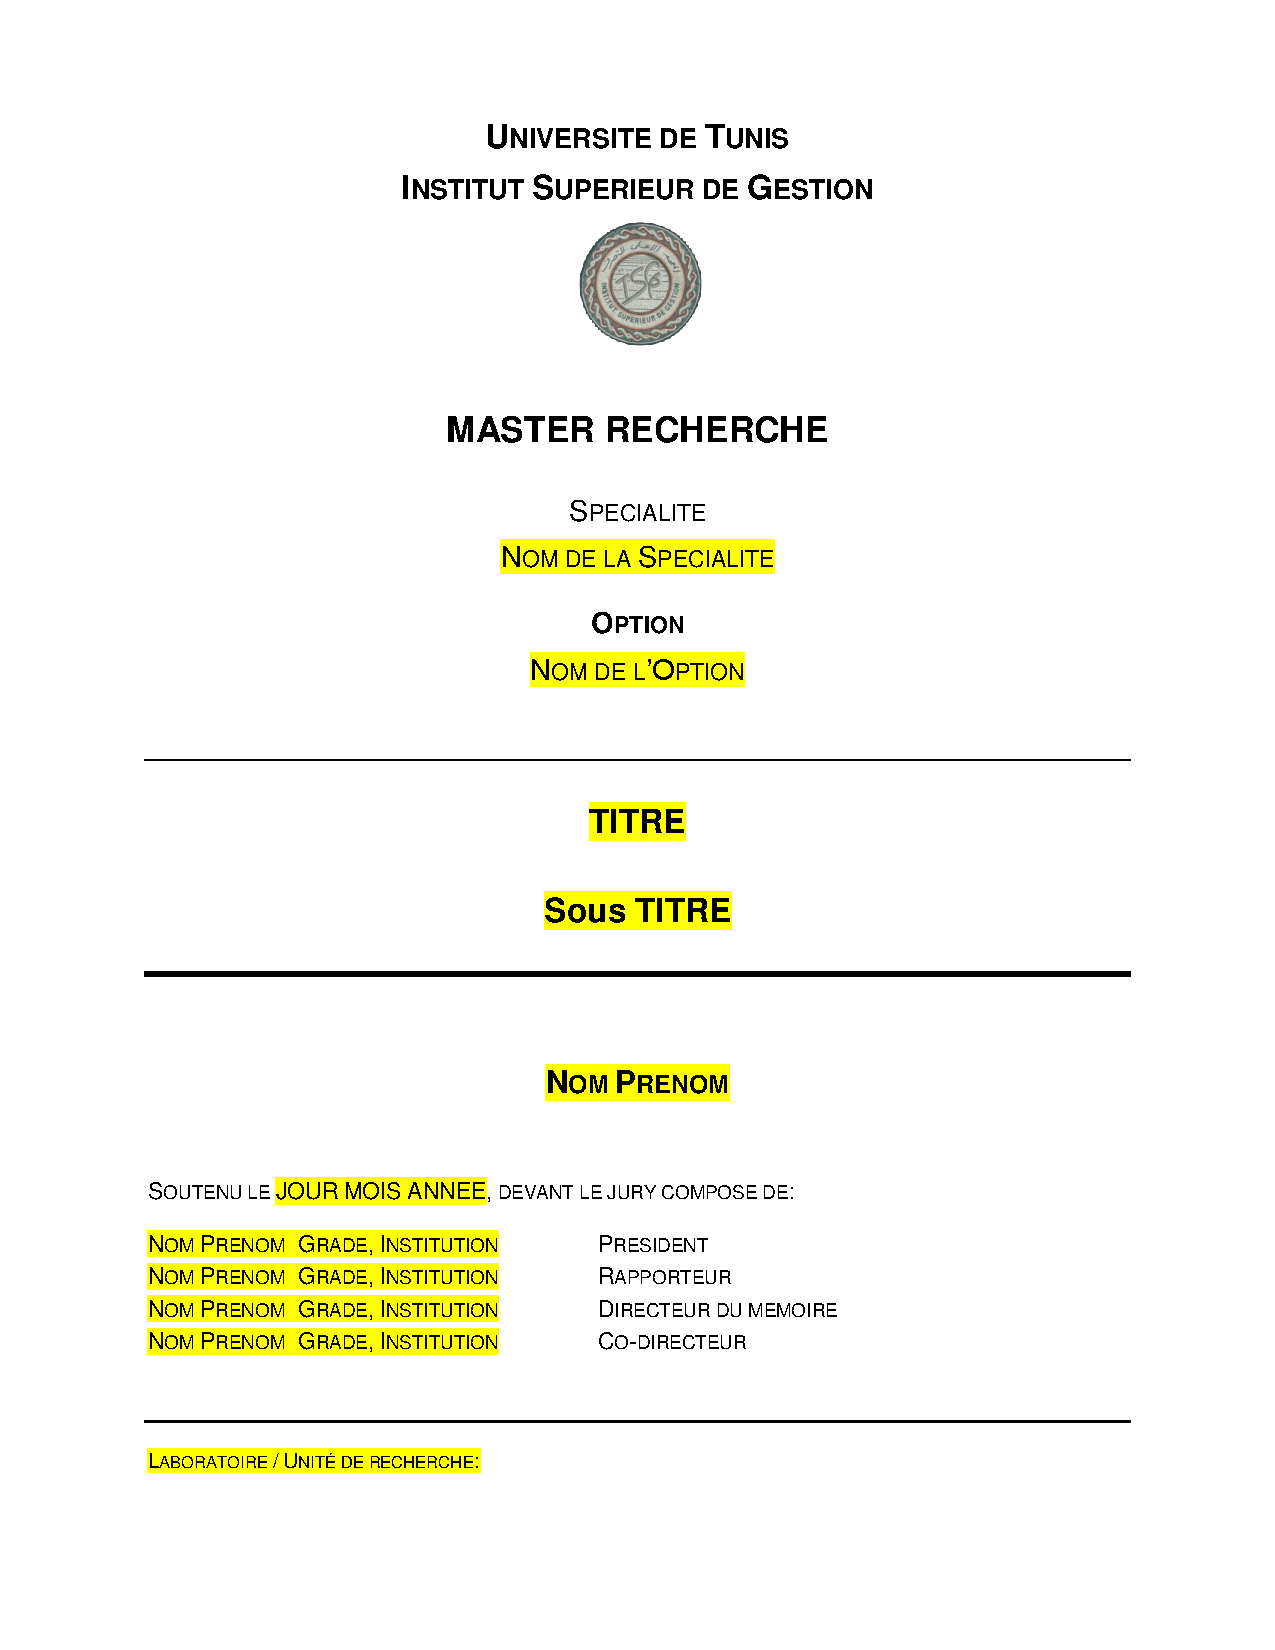
\includepdf{PageDeGarMaster.pdf}
\begin{center}
\thispagestyle{empty}
\vspace{-3cm}
\center{\large{\textsc{Universit\'e de Manouba}}}
\vspace{-0.3cm}
\center{\large{\textsc{Institut Sup\'erieur des Arts Multim�dia}}}
\begin{figure} [H]
\begin{center}

\includegraphics [width=2.5cm]{91.png}
\end{center}
\end{figure}
\vspace{-0.5cm}






{\Large{\textsc{Achievement of the requirement of the degree of
Diploma in Computer Science and Multimedia Engineering}}}

\center{\textsc{Specialty}}
\vspace{-0.4cm}
\center{\small{\textsc{Computer Science and Multimedia}}}
\center{\textsc{Option}}
\vspace{-0.4cm}
\center{\small{\textsc{Software engineering}}}
%pour Sciences et Techniques de l'Informatique D�cisionnelle (STID) 3 options
%\center{\small{\textsc{Informatique et Gestion de la Connaissance (IGC)}}}
%\center{\small{\textsc{M�thodes intelligentes pour l'aide � la d�cision (MIAD)}}}
%\center{\small{\textsc{Statistical Machine Learning (SML)}}}
%pour Gestion 2 options
%\center{Marketing (MKT)}
%\center{Administration et strat�gie des affaires (ASA)}
% pour Mod�lisation 2 options
%\center{\small{Aide � la d�cision}
%\center{\small{Pr�vision}
\vspace{1cm}
\hrule height 1pt
\center{\textbf{\large{Analysis of twitter data on sustainable development goals}}} % en maj
\vspace{1cm}
\\ \par
\hrule height 4pt
\par
\vspace{1cm}
\center{\large{\textsc{Ines Aouadi}}}
\vspace{0.5cm}




\begin{table} [H]
\renewcommand{\footnoterule}{}
\renewcommand{\arraystretch}{1}
\setlength\tabcolsep{5pt}
\begin{tabular}{lll}
\\  \multicolumn{3} {l} {\small{\textsc{Pedagogic advisors :}}}
 \\ \\ \textsc{Sehl Melouli}  & \textsc{professor, LAVAL UNIVERSITY}
  \\ \textsc{Tarek Hamrouni}  & \textsc{professor, High Institute of Arts Multimedia} 

\\ \vspace{0.5cm}
\end{tabular}
\end{table}

\hrule
%\center{\footnotesize{2013-2014}}






\end{center}
 \footnotesize{Research Unit: Centre de Recherche sur les Communaut\'es Intelligentes }  %� supprimer si le m�moire n'est pas effectu� dans un laboratoire ou une unit� 
\clearpage
\thispagestyle{empty}
\cleardoublepage
 \newpage
\normalsize





 \newpage
\def\cleardoublepage{\clearpage
 \if@twoside
  \ifodd\c@page\else
   \null\thispagestyle{empty}\newpage
   \if@twocolumn\null\newpage\fi
   \fi
  \fi
 }%
\def\ps@chapterverso{\ps@empty}%
\tableofcontents
\newpage
\def\cleardoublepage{\clearpage
 \if@twoside
  \ifodd\c@page\else
   \null\thispagestyle{empty}\newpage
   \if@twocolumn\null\newpage\fi
   \fi
  \fi
 }%
\def\ps@chapterverso{\ps@empty}%
%%%% fin macro %%%%


\cleardoublepage
%\newpage
\thispagestyle{empty}
\listoffigures
\cleardoublepage
\newpage
\listoftables
\newpage
 \cleardoublepage
\listofalgorithms
 \newpage
\def\cleardoublepage{\clearpage
 \if@twoside
  \ifodd\c@page\else
   \null\thispagestyle{empty}\newpage
   \if@twocolumn\null\newpage\fi
   \fi
  \fi
 }%
\def\ps@chapterverso{\ps@empty}%
%%%% fin macro %%%%


\cleardoublepage
%\newpage
\thispagestyle{empty}



\pagenumbering{arabic}
 
\chapter*{Introduction} \markboth{Introduction}{Introduction}


   \newpage
\def\cleardoublepage{\clearpage
 \if@twoside
  \ifodd\c@page\else
   \null\thispagestyle{chapterverso}\newpage
   \if@twocolumn\null\newpage\fi
   \fi
  \fi
 }%
\def\ps@chapterverso{\ps@empty}%
%%%% fin macro %%%%

\chapter{General context}
\section{Introduction}
During this introductory chapter, we will talk about the Problematic and we will try to define the challenges and constraints of our project.Later, we will explain our objectives in order to accomplish our mission. Finally, we will end this section with a presentation of the framework of our internship.
\section{Problematic}
The concept of “smart city” is evolving as a new approach to mitigate and remedy current urban problems and make urban development more sustainable \cite{Alawadhi2012}.in this case, we must have citizen with operational feedback.\\
We focus on twitter microblog to extract  information.This platform is accessible through websites or cellphone applications allowing users to instantly post relevant information about what they are seeing, hearing and experiencing around them. In a SDG case, such platform provide valuable information shared voluntary to inform or alert the society .\\
Information retrieval from microblogs is hindered by many challenges such as: streaming data analysis,the variety of information format and language processing, large datasets, and extracting relevant and fresh information from a huge amount of outdated and redundant data.
\section{Objectives}
The objective of the proposed research is to provide insights on the online interactions and revealed perceptions of stakeholders about the SDG related to cities. We will provide cities with new informational tools, supporting their strategy in order to achieve the SDG11
(sustainable cities and communities) goal and its targets. 
\\
These informational tools will enable to bridge the gap between the vision of the diverse stakeholders, from United Nations, government and non-government agencies, to the civil society and the private sector. Specifically, the proposal will analyze the data posted on the Twitter platform to provide agencies and citizens with operational feedback on how SDGs are perceived and implemented.
\section{framework of our internship}
The internship is on the context of obtaining of the degree of Diploma in Computer Science and Multimedia Engineering.
\\
The internship was proposed by CeRCI Unit. It have an overall duration of four months. 
 \begin{itemize}
 \item Phase of documentation and bibliographic study which have a duration of one month.
 \item Phase of development and experimentation which was concertized by a practical internship in the laboratory CeRCI at  Laval University with two months of work.
 \item Phase of The synthesis and evaluation of the  obtained results which was elaborated in one month.
 \end{itemize} 
\subsection{laboratory CeRCI}
Laboratory CeRCI,Intelligent Communities Research Center,was created in XXXX in Laval University.
\begin{figure} [H]
\begin{center}

\includegraphics [width=2.5cm]{logo.png}
\caption{Logo Laval University}
\end{center}
\end{figure}
\textbf{Organizational chart}

Laboratory CeRCI was founded by five professors: Sehl Mellouli, Monia Rekik, Adnène Hajji, Jacqueline Corbett et Karim Ben Boubaker.
The research activities is centered  to three axes: citizen, governance and technology.  
\section{Conclusion}
During this chapter, we have presented the project, the framework of internship and the work obligations. In the next chapter,we will present and compare the commonly used approach  of information retrieval.


 \newpage
\def\cleardoublepage{\clearpage
 \if@twoside
  \ifodd\c@page\else
   \null\thispagestyle{chapterverso}\newpage
   \if@twocolumn\null\newpage\fi
   \fi
  \fi
 }%
\def\ps@chapterverso{\ps@empty}%
%%%% fin macro %%%%


\chapter{State of the art}
\section{Introduction}
This section aims at introducing micro blog platform ,SDG  and information retrieval in order to provide the reader with basic notions and necessary technical background to understand in more details next chapters. 
\section{Sustainable development goals}
The Sustainable Development Goals (SDGs), otherwise known as the Global Goals, are a universal call to action to end poverty, protect the planet and ensure that all people enjoy peace and prosperity.\footnote{https://sustainabledevelopment.un.org/} 
On September 25th 2015,the 194 countries of the UN General Assembly adopted the 2030 Development Agenda titled Transforming our world: the 2030 Agenda for Sustainable Development.Countries adopted those goals which are a set of 17:
\begin{enumerate}
\item No Poverty
\item Zero Hunger 
\item Good Health and Well-Being
\item Quality Education
\item Gender Equality
\item Clean Water and Sanitation
\item Affordable and Clean Energy
\item Decent work and Economic Growth
\item Industry, Innovation and Infrastructure
\item Reduced Inequality
\item Sustainable Cities and Communities
\item Responsible Consumption and Production
\item Climate Action
\item Life Below Water
\item Life On Land
\item Peace, Justice and Strong Institutions
\item Partnerships for the goals
\end{enumerate}
The SDGs work in the spirit of partnership and pragmatism to make the right choices now to improve life, in a sustainable way, for future generations. They provide clear guidelines and targets for all countries to adopt in accordance with their own priorities and the environmental challenges of the world at large.To make a positive change for both people and planet,They tackle the root causes of poverty and unite us together.
\section{Microblogs Platform}
Nowadays, everyone can easily share and access to content on the web within few second.According to internet live stats website, 90\% of information shared daily on the web is essentially provided from microblogging platforms\footnote{http://www.internetlivestats.com/} .
\\Data acquisition and extraction from microblogging platforms is being an important research field. We focus on analyzing extraction and acquisition techniques adapted to the microblogging platform Twitter cause this is platform is one of the most popular microblog platforms according a large set of rich information shared and updates publicly regarding various topics and events.
\\With around 500 million of daily shared tweets,Twitter microblogging platform is ranked in the second position.Such shared information are generally not provided by search engines websites as they are usually not yet indexed and thus available only through the microblogging platform search tools.
\\The wealth of information shared in Twitter is attracting an increasing attention of researchers in many fields especially knowledge discovery and data mining.Exploring such information qualitatively and quantitatively could lead to understand and propose new powerful models learning the particularities of human behavior and interests.
\subsection{Twitter Microblog}
Twitter was created in March 2006 by Jack Dorsey, Evan Williams, Biz Stone, and Noah Glass and launched in July 2006. Twitter allows users  to publish messages, known as tweets, expressed with no more than 140 characters via SMS or web or/and mobile applications. 
\\Nowadays, Twitter has gained a huge popularity. In our daily life, we used twitter  to comment on any news and discuss trending topics. It has integrated richer characteristics by enabling users to publish various data content formats such as texts, images, links and videos.
Twitter combines elements of social network sites and blogs , but with a few notable differences.
\begin{figure} [H]
\begin{center}

\includegraphics [width=2.5cm]{tweet.png}
\caption{Logo Twitter}
\end{center}
\end{figure}
\vspace{-0.5cm}
\textbf{specificity of Tweets}
\\
\textit{Usernames:}
In order to direct their messages users often include twitter usernames in their tweets. A de facto standard is to include @ symbol before the username (e.g.@towardshumanity). 
\\
\textit{Usages of links:}
Users very often include links in their tweets.(only 140 characters)
\\
\textit{Stop words:}
There are a lot of stop words or filler words such as “a”, “is”, “the” used in a tweet which does not indicate any sentiment or meaning.
\\
\textit{Repeated letters:}
Tweets contain very casual language. For example,  “hello” with an 
helloooo,helllo 
\section{Data Collection Technique}
\subsection{Direct Data Access}
\textbf{Data Access via Research Data Collections:}
Test collections are generally composed of a set of documents related to one or various topics suited to specific information needs.\\
\textbf{Data Access via US Congress Library:}
Since April 2010, the Library of Congress has announced its intention to archive public historic tweets for conservation and research.\\
\textbf{Data Access via Data Grants:}
Twitter has introduced,in February 2014, its Data Grants project accepting applications from any member of research institutions to access to the needed historical and public information required in their research studies.
\subsection{Data Access via Ad-hoc Applications}
\textbf{Data Access via Public Twitter APIs}\\
\textbf{Data Access via Crawling Techniques}
\section{Natural Language Processing}
Natural Language Processing (NLP) is an area of research and application that explores how computers can be used to understand and manipulate natural language text. NLP researchers aim to collect knowledge on how human beings understand and use language so that fitting tools and techniques can be developed to make computer systems understand and manipulate natural languages to perform the preferred tasks.
\subsection{Steps in NLP}
NLP includes five general Steps:
\begin{itemize}
\item Lexical Analysis: it means dividing the whole text into paragraphs, sentences and words. It is analyzing the structure of words. 
\item Syntactic Analysis: It implicates analysis of words in the sentence for grammar and arrangement of words in a manner that shows the relationship among the words.
\item Semantic Analysis:  It defines the exact meaning or the dictionary meaning from the text.
\item Disclosure Integration: The meaning of any sentence depends upon the meaning of the sentence just before and after it.
\item Pragmatic Analysis: It involves deriving those aspects of language which require real world knowledge.
\end{itemize}
\section{Information Retrieval}
Information retrieval is the science of searching for information in a document, searching for document themselves, searching for metadata that describe data and for databases such as text, image or sound.
\subsection{IR based on Information Content Classification}
classification strategy consists of analyzing tweets content for
situational information retrieval. Many classification dimensions have been explored to separate between relevant and irrelevant situational information:
\\
\textbf{location}\\
\textbf{time}\\
\textbf{Credibility}\\
\textbf{Information provided}
\subsection{IR based on Information Providers Classification}
classification strategy consists of identifying the prominent microblog
users who are susceptible to provide the targeted relevant information
\\
\textbf{User's connectivity graph}
\\
\textbf{User's interaction graph}
\\
\textbf{User's activities}
\section{Approaches analysis Tweets}
Many models were proposed to analyze tweets such are:
\begin{itemize}
\item TF-idf(term preponderate)
\item LDA(probabilistic)
\item Vector space model or term vector model
\item LSA(latent semantic analysis)(presentation term and document in the same space : improvement of Vector space model)
\end{itemize}
\section{Conclusion}
NLP is a powerful tool if understood and properly used.In the next chapter, we will discuss our contribution in order to extract meanings and links between the tweets collected





 \newpage
\def\cleardoublepage{\clearpage
 \if@twoside
  \ifodd\c@page\else
   \null\thispagestyle{chapterverso}\newpage
   \if@twocolumn\null\newpage\fi
   \fi
  \fi
 }%
\def\ps@chapterverso{\ps@empty}%
%%%% fin macro %%%%
\newpage
\cleardoublepage




\chapter*{Conclusion}

 \markboth{Conclusion}{Conclusion}

\addcontentsline{toc}{chapter}{Conclusion}


 \newpage
\def\cleardoublepage{\clearpage
 \if@twoside
  \ifodd\c@page\else
   \null\thispagestyle{chapterverso}\newpage
   \if@twocolumn\null\newpage\fi
   \fi
  \fi
 }%
\def\ps@chapterverso{\ps@empty}%
%%%% fin macro %%%%

%%%% fin macro %%%%



%\nocite{*}
\bibliographystyle{Apacite}
\bibliography{NewBib}


\end{document}

